\subsection{Matrix dimension L=2}

OBS! Need an number of MC cycles necessary!

All calculations in this subsection are at T = 1.0 K. 

\begin{table}\caption{This table compares the analytical values for L=2 with the numerical ones after $10^6$ Monte Carlo cycles. The values are in units per spin.}\label{tab:compare_values}
\begin{tabular}{ccc}
& Numerical: & Analytical:\\ \hline
$\left<E\right>$ &   -1.9958 & -1.9960\\
$\left<E^2\right>$ &   15.9664 & 15.9679\\
$\left<M\right>$ &    0.0451 & 0\\
$\left<M^2\right>$ &    3.9930 & 3.9933\\
$\left<|M|\right>$ &    0.9986 & 0.9987\\
$\chi$ &   3.9849 & 3.9933\\
  $C_V$& 0.0335 & 0.0321\\
\end{tabular}
\end{table}

\begin{figure}[H]
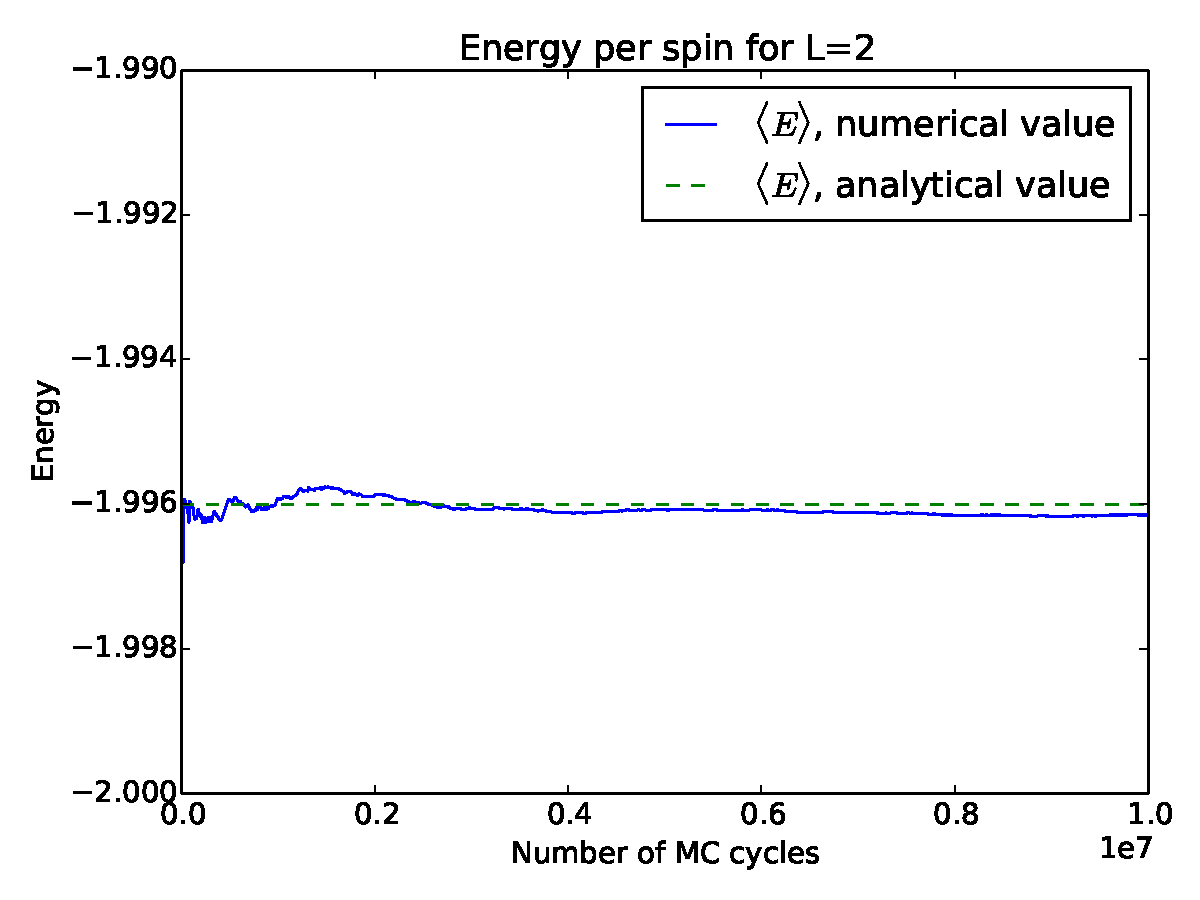
\includegraphics[width=\linewidth]{../results/4b/L_2_energy}\caption{This is a plot of the expectation value of the energy per spin verus number of Monte Carlo cycles. The plot shows that at least $ 9 \cdot 10^{5} $ MC cycles are necessary for a good argeement.}\label{fig:L_2_energy}
\end{figure}

\begin{figure}[H]
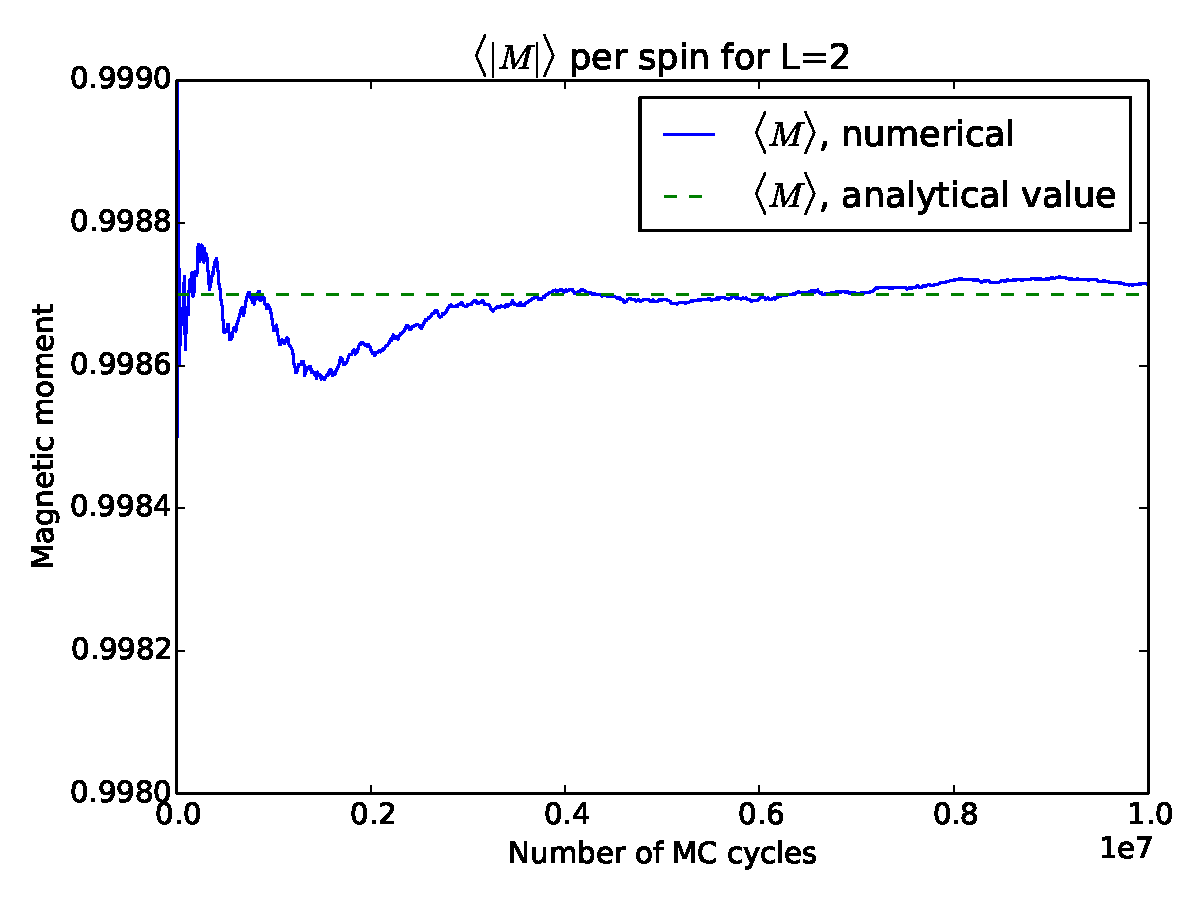
\includegraphics[width=\linewidth]{../results/4b/L_2_magnetic_abs}\caption{This is a plot of the expectation value of the mean absolute value of the magnetic moment per spin verus number of Monte Carlo cycles. The plot shows that at least $ 8 \cdot 10^{5} $ MC cycles are necessary for a good argeement, but all the way to $10^6$ the value is a bit low.}\label{fig:L_2_magnetic_abs}
\end{figure}

\begin{figure}[H]
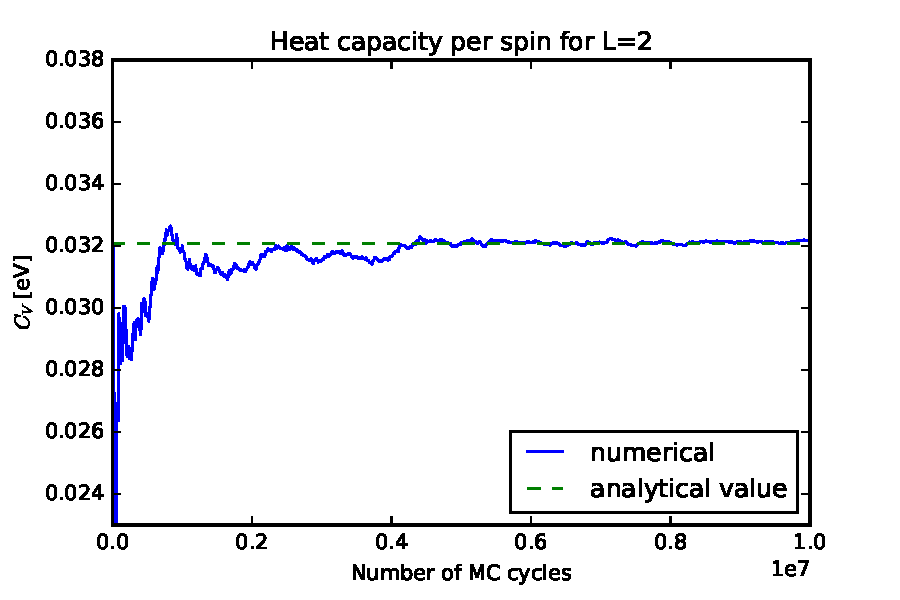
\includegraphics[width=\linewidth]{../results/4b/L_2_heat_capasity}\caption{This is a plot of the heat capacity per spin verus number of Monte Carlo cycles. The plot shows that at least $ 6 \cdot 10^{5} $ MC cycles are necessary for a good argeement.}\label{fig:L_2_heat_capacity}
\end{figure}

\begin{figure}[H]
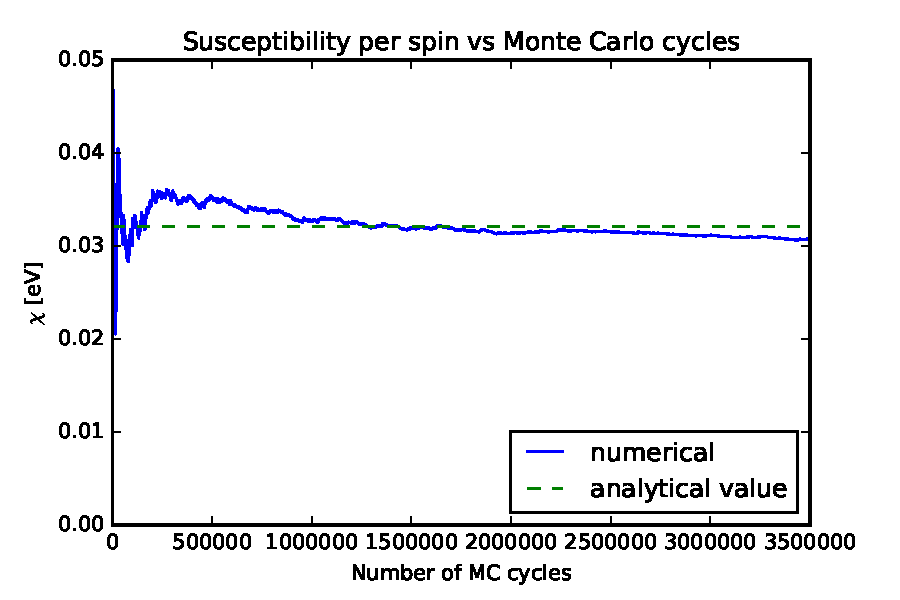
\includegraphics[width=\linewidth]{../results/4b/L_2_susceptibility}\caption{This is a plot of the susceptibility per spin verus number of Monte Carlo cycles. The plot shows that at least $ 6 \cdot 10^{5} $ MC cycles are necessary for a good argeement.}\label{fig:L_2_susceptibility}
\end{figure}

\subsection{Matrix dimension L = 20}

HMM: Should define an area that is enough for equilibrium!

OBS: Need the number of MC cycles to reach equilibrium!

OBS: Need equilibration time! (5 1e5?)

OBS: Comment accepted configs T dependency

\begin{figure}[H]
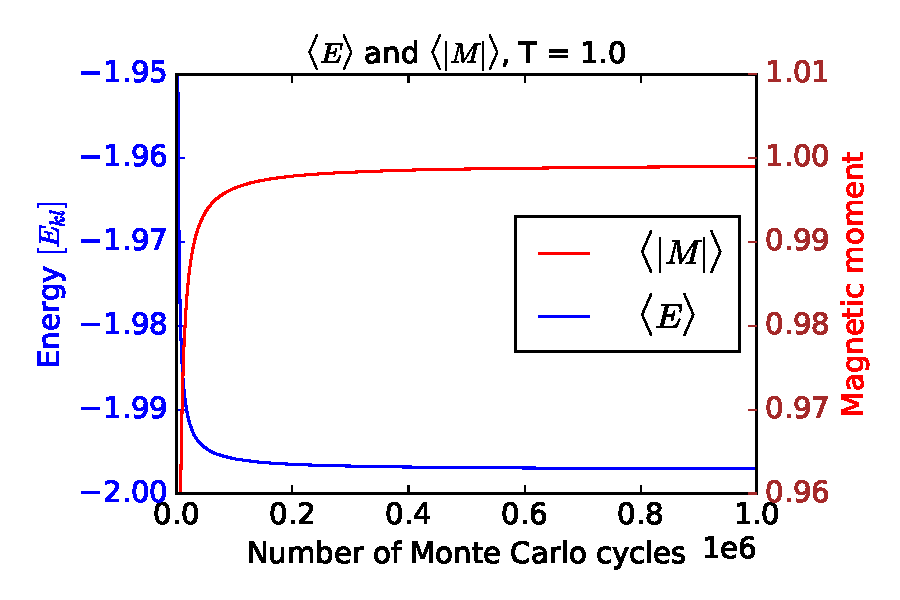
\includegraphics[width=\linewidth]{../results/4c/En_mag_T1_0}\caption{This is a plot of both the expectation value of the energy and absolute magnetic moment per spin verus number of Monte Carlo cycles at T = 1.0 K. The plot shows that at least \ref MC cycles are necessary to reach equilibrium.}\label{fig:L_20_energy_mag_T_1.0}
\end{figure}

\begin{figure}[H]
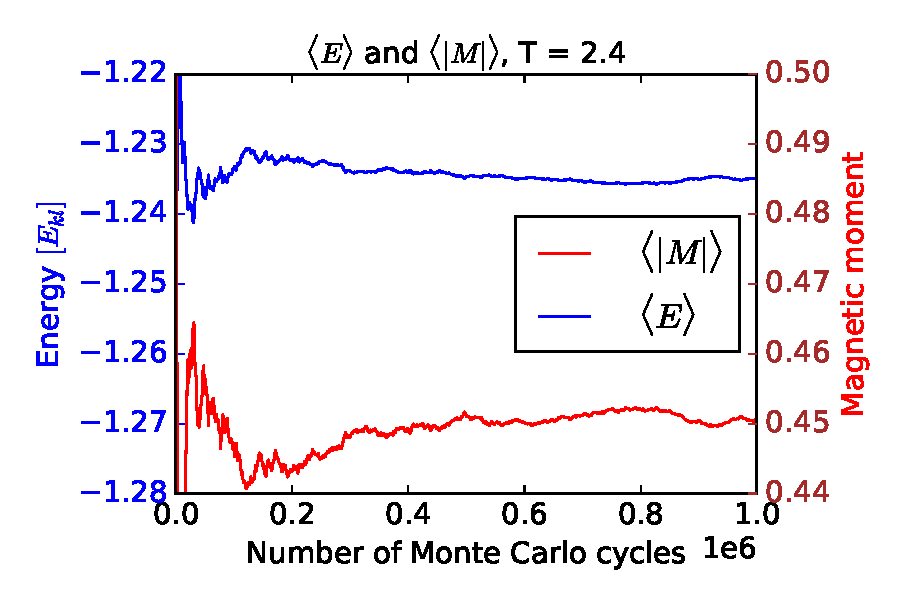
\includegraphics[width=\linewidth]{../results/4c/En_mag_T2_4}\caption{This is a plot of both the expectation value of the energy and absolute magnetic moment per spin verus number of Monte Carlo cycles at T = 2.4 K. The plot shows that at least \ref MC cycles are necessary to reach equilibrium.}\label{fig:L_20_energy_mag_T_2.4}
\end{figure}

\begin{figure}[H]
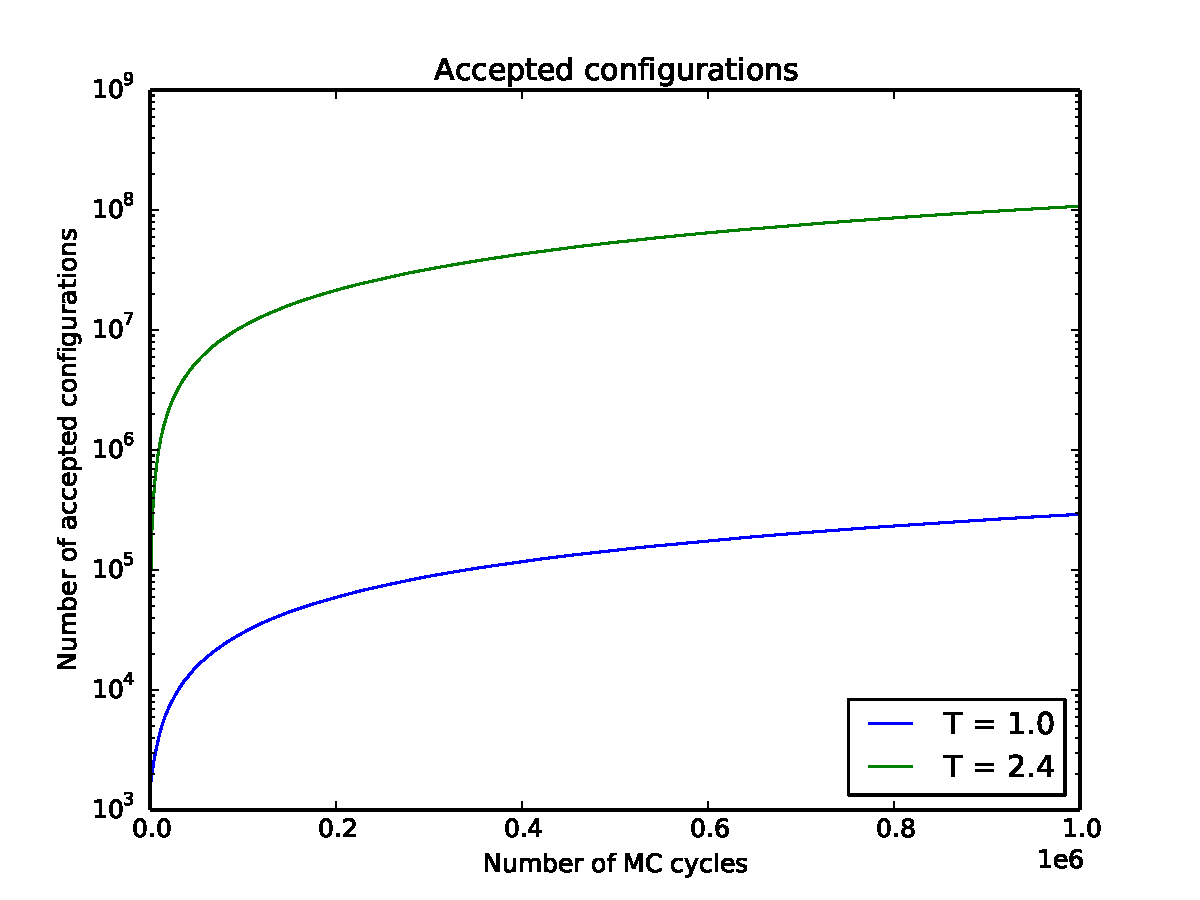
\includegraphics[width=\linewidth]{../results/4c/L_20_accepted_configs_}\caption{This is a plot of the total number of accepted configurations versus number of Monte Carlo cycles with random initial state.}\label{fig:total_accepted}
\end{figure}

\begin{figure}[H]
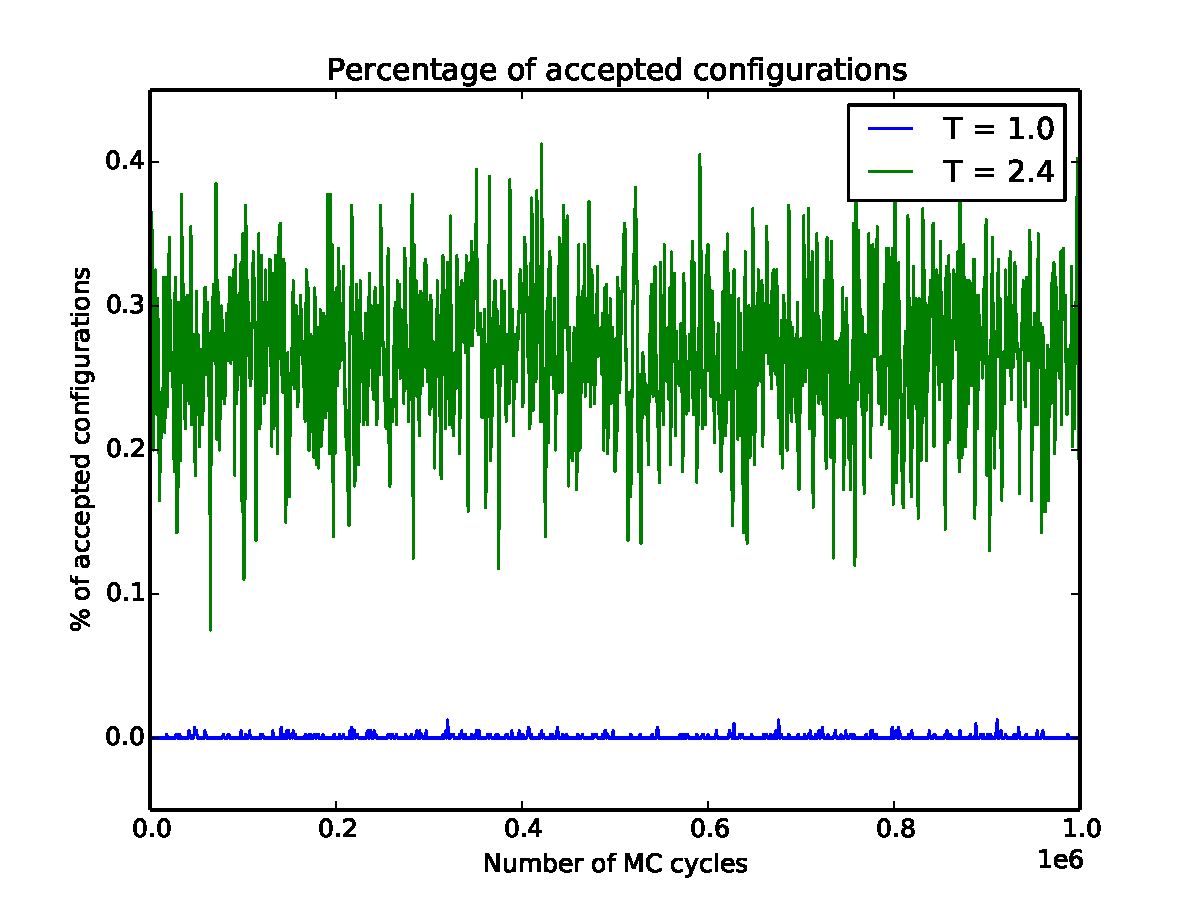
\includegraphics[width=\linewidth]{../results/4c/L_20_accepted_configs}\caption{This is a plot of the percentage accepted of attempted configurations versus  Monte Carlo cycles with random initial state.}\label{fig:percentage_accepted}
\end{figure}

\subsection{Energy probability}

OBS: Compare result with computed variance!

OBS: Discuss behavior (In Discussion - maybe just merge result and discussion?)

Computed variance (from same dataset?):

$$ \sigma_E^2 = \left< E^2\right> - \left< E\right>^2 $$

T = 1.0 K:

$$ \sigma_E^2 = 1595.45 - (-1.997)^2 = 1591.46$$

T = 2.4 K:

$$ \sigma_E^2 =   620.734 - (-1.23759)^2
 = 619.20$$

\begin{figure}[H]
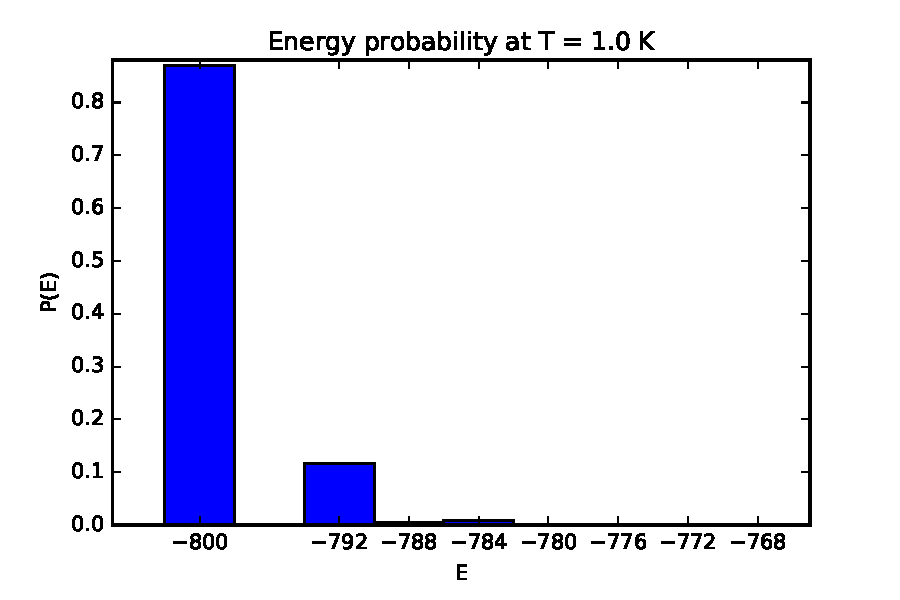
\includegraphics[width=\linewidth]{../results/4d/d_T_1probability}\caption{This is a plot of the energy probability when T = 1.0 K.}\label{fig:probability_T_1.0}
\end{figure}

\begin{figure}[H]
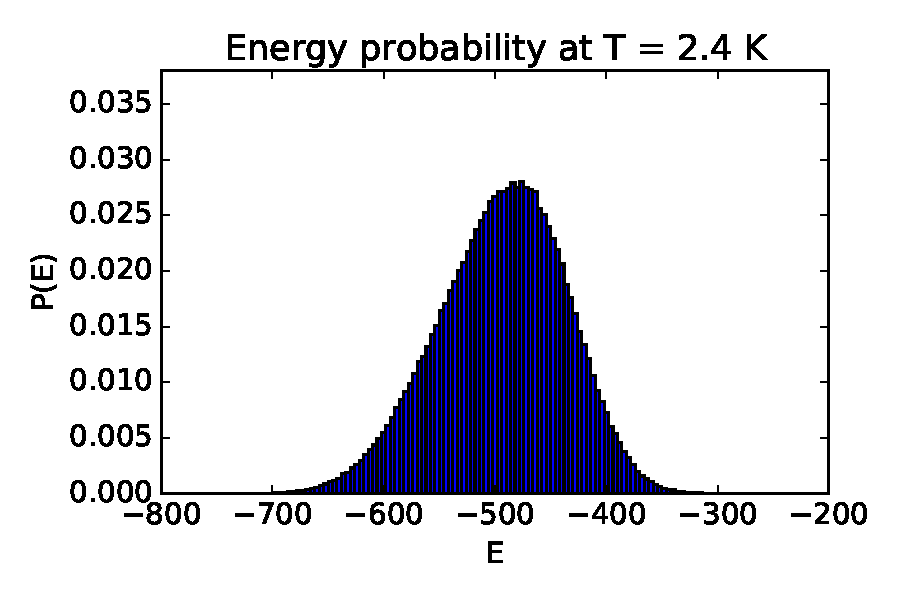
\includegraphics[width=\linewidth]{../results/4d/d_T_2_4probability}\caption{This is a plot of the energy probability when T = 2.4 K.}\label{fig:probability_T_2.4}
\end{figure}

\subsection{Increasing dimensionality/ Critical temperature}

OBS: Plot of E, M, Cv, X as functions of T (put L as legend and plot together)

OBS: Indication of phase transition? (Peak - at least for Cv and X)

OBS: Use Equation \ref{eq:critical_T} to extract $T_C$.